\section{Code availability}\label{app:code}

The two-dimensional ice flow model is written in python and the entire project can be found in an \href{https://gitlab.met.fu-berlin.de/rw0064fu/glaciology}{online repository}\footnote{\hypersetup{urlcolor=}\url{https://gitlab.met.fu-berlin.de/rw0064fu/glaciology}}. The ice transport equations are numerically solved in the main model part found in \code{2d-ice-sheet/2d\_model.py}, while the SMB is externally computed and updated in the \code{2d-ice-sheet/surface\_mass\_balance.py} file. The corresponding parameters for initializing the temperature and precipitation fields are stored in the \code{params.py} files in the respective subdirectories.

\section{SMB parametrization}\label{app:era5}

In order to derive an estimate for the values of the different scaling methods in \cref{tab:smb}, multi-year plots of the mean
temperature (\cref{fig:era5}) and precipitation (\cref{fig:era5-pr}) in Greenland are created based on ERA5 reanalysis data from 2010 to 2019.

\begin{figure}[h]
	\centering
	\begin{subfigure}{0.49\textwidth}
		\centering
		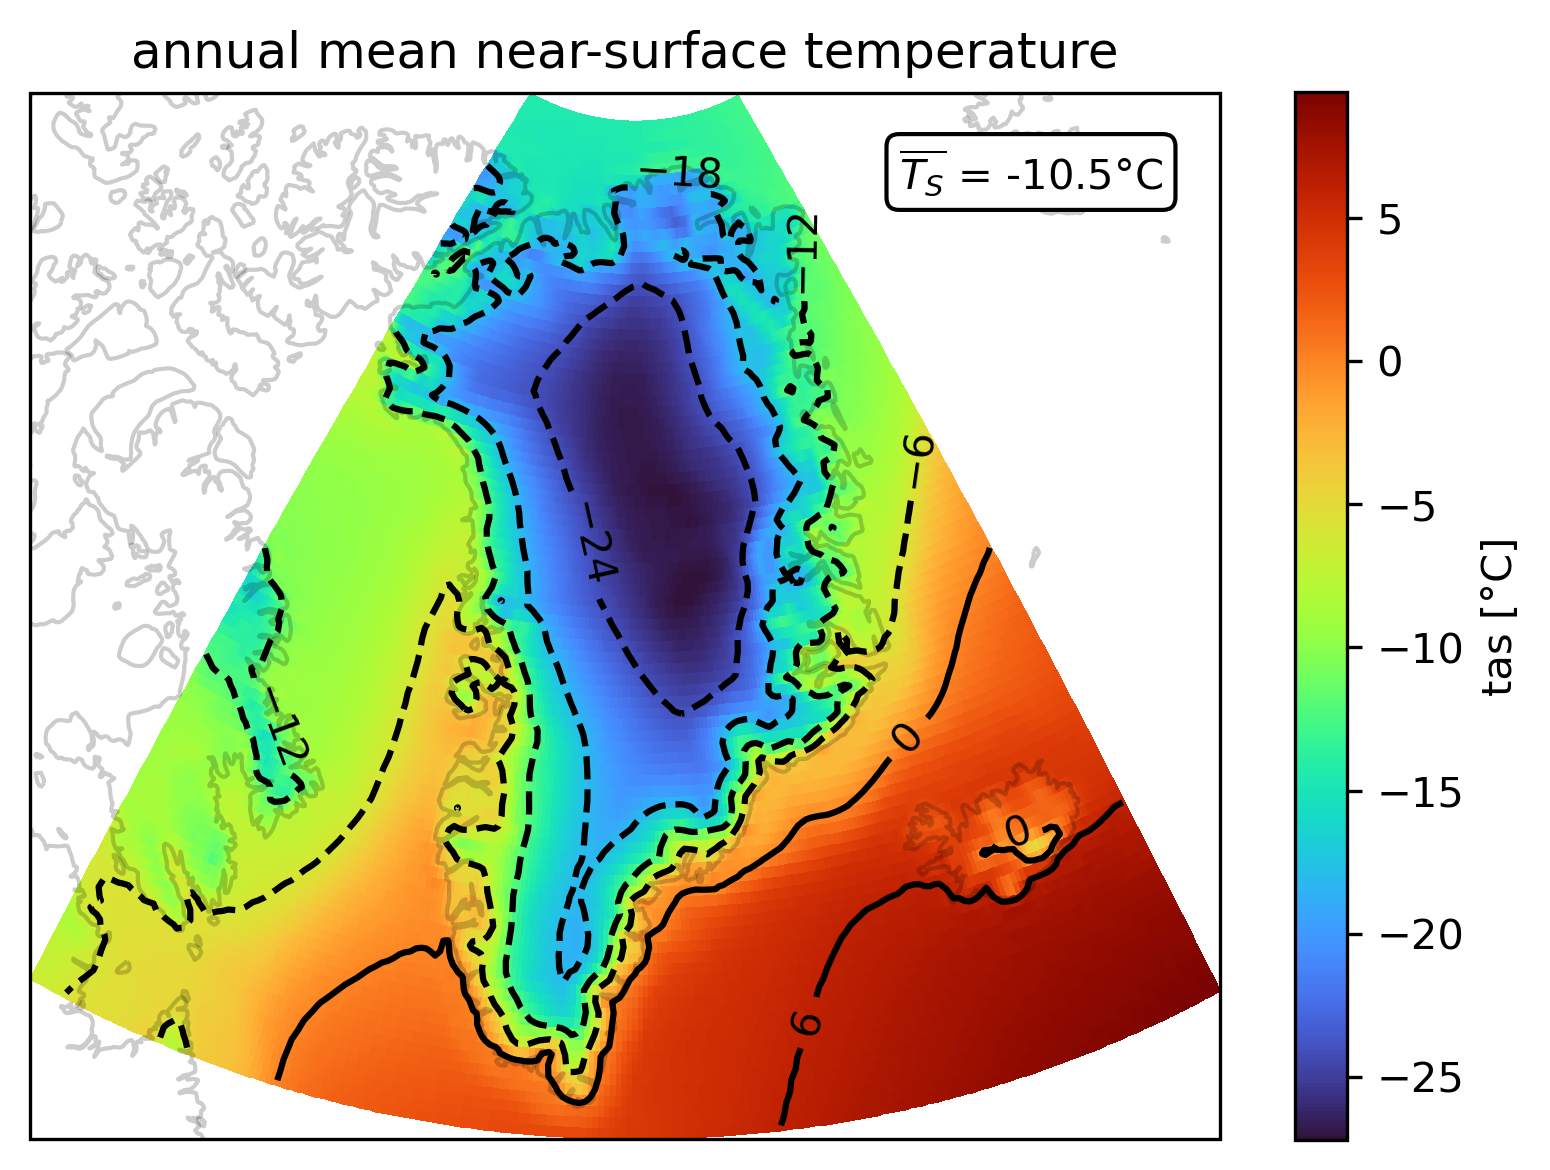
\includegraphics[width=\textwidth]{../../era5/figs/tas-annual-mean.png}
	\end{subfigure}
	\begin{subfigure}{0.49\textwidth}
		\centering
		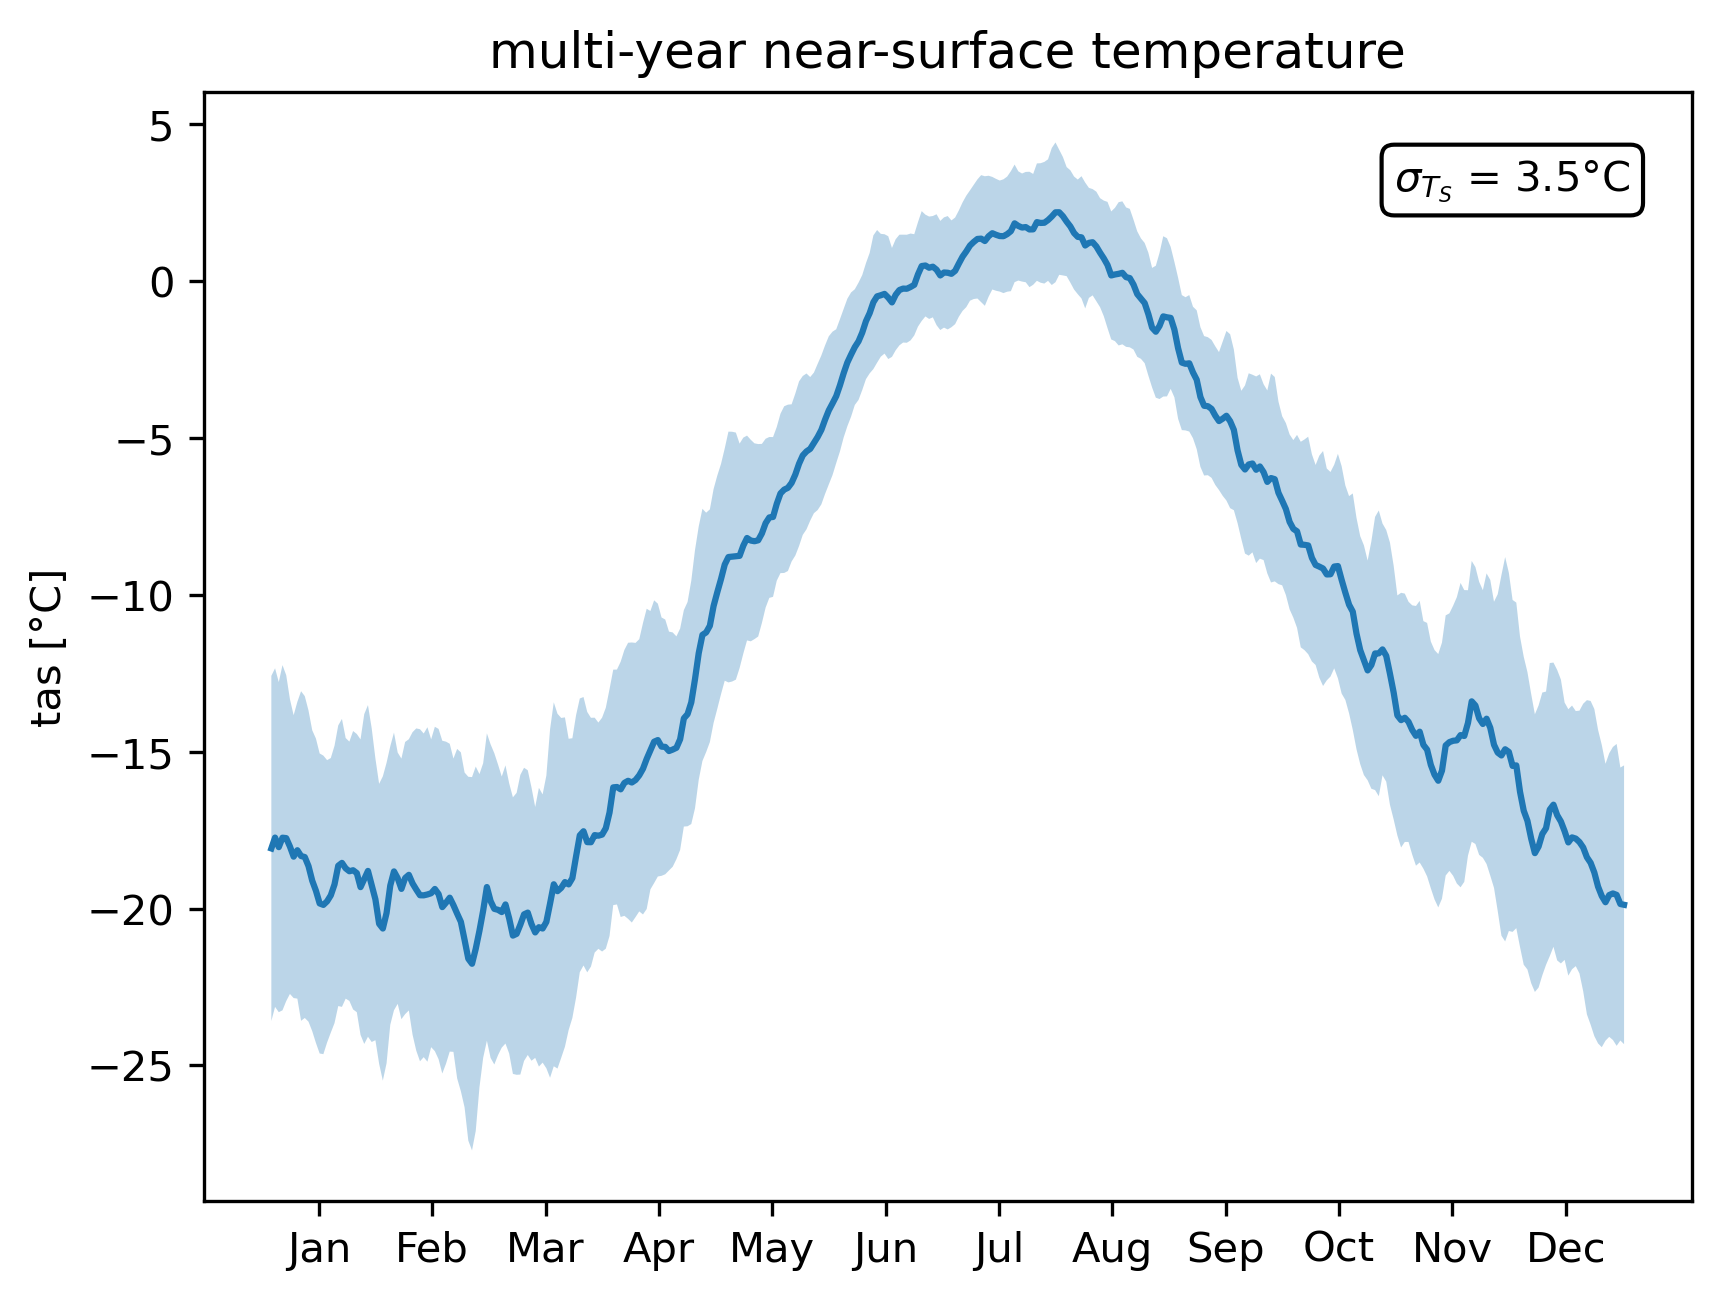
\includegraphics[width=\textwidth]{../../era5/figs/tas-seasonality.png}
	\end{subfigure}
	\caption{Spatial distribution and seasonality of temperature field}
	\label{fig:era5}
\end{figure}

\begin{figure}
	\centering
	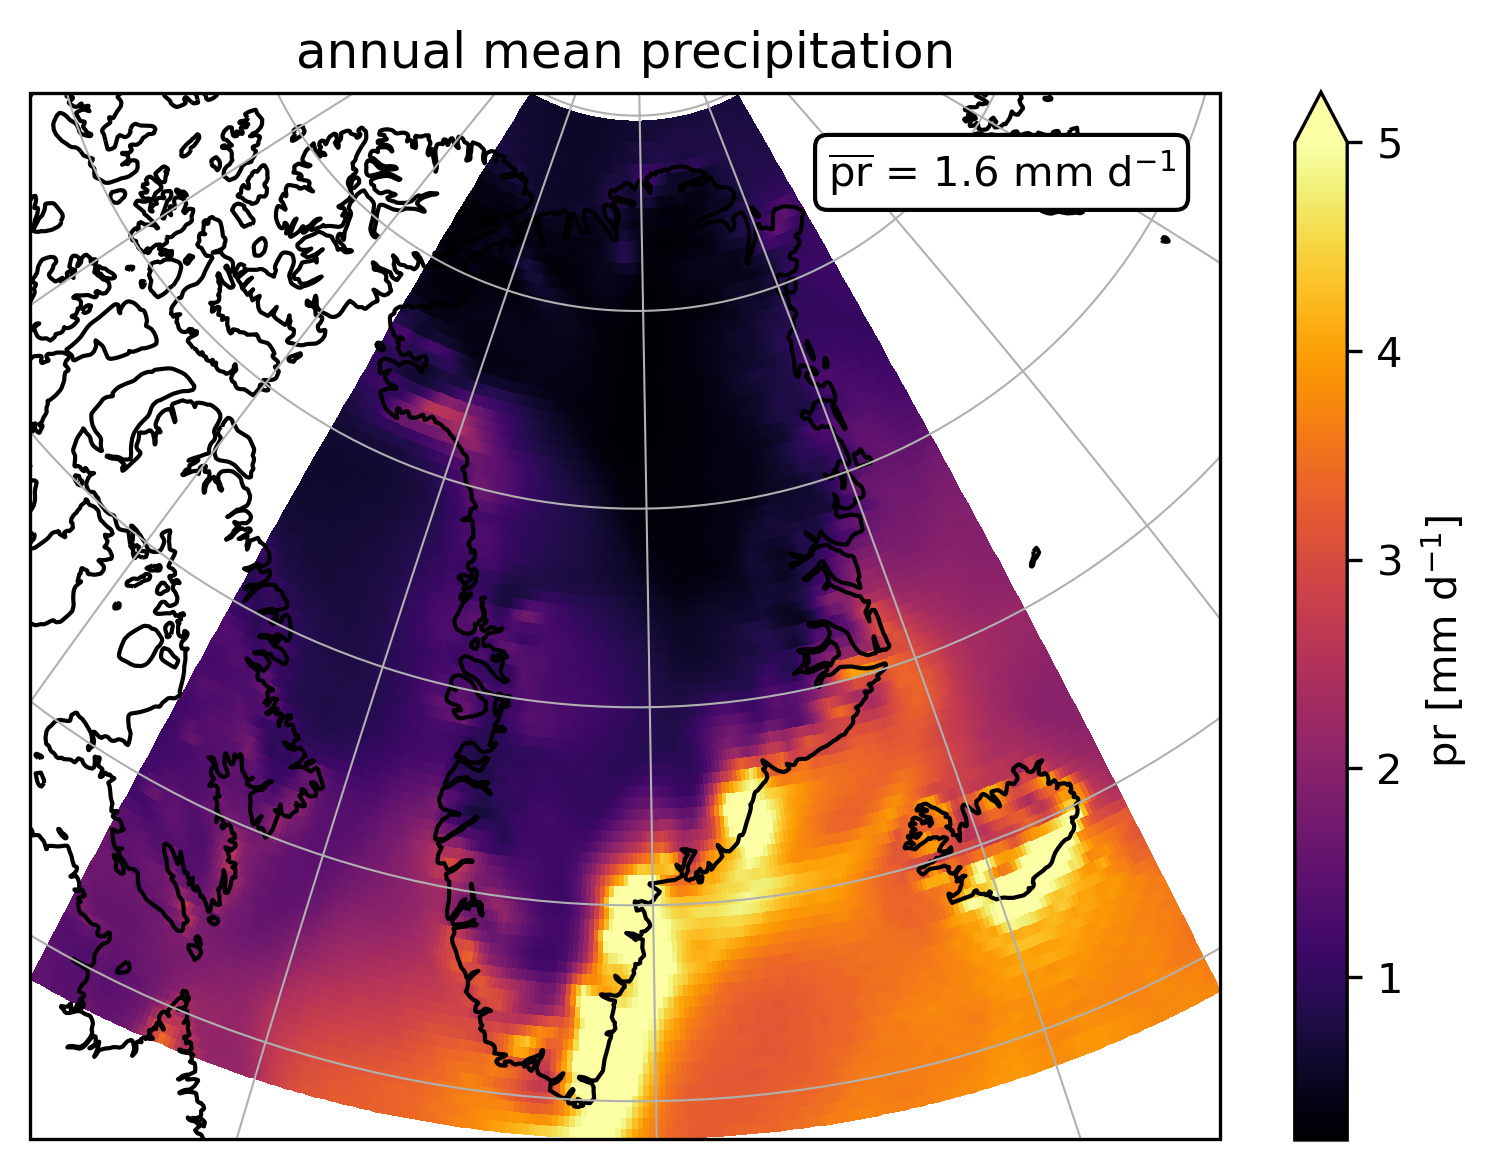
\includegraphics[width=0.6\textwidth]{../../era5/figs/pr-annual-mean.png}
	\caption{Precipitation field; the maximum annual precipitation is \(\mean{P}_{\text{max}} = \SI{8.84}{\mm\per\day}\) (not displayed by cropped colorbar)}
	\label{fig:era5-pr}
\end{figure}

\section{Climate forcings}

\subsection{NorESM}\label{app:forcing-noresm}

The NorESM climate forcing depends on a future projection of the climatology, scaled by a climate index (\cref{fig:climate-index}) to match the respective year of the simulation. For roughly the first \SI{200}{\year}, the climate index increases, until reaching a constant value of \(\approx\num{3}\) for the remaining time.  

\begin{figure}
	\centering
	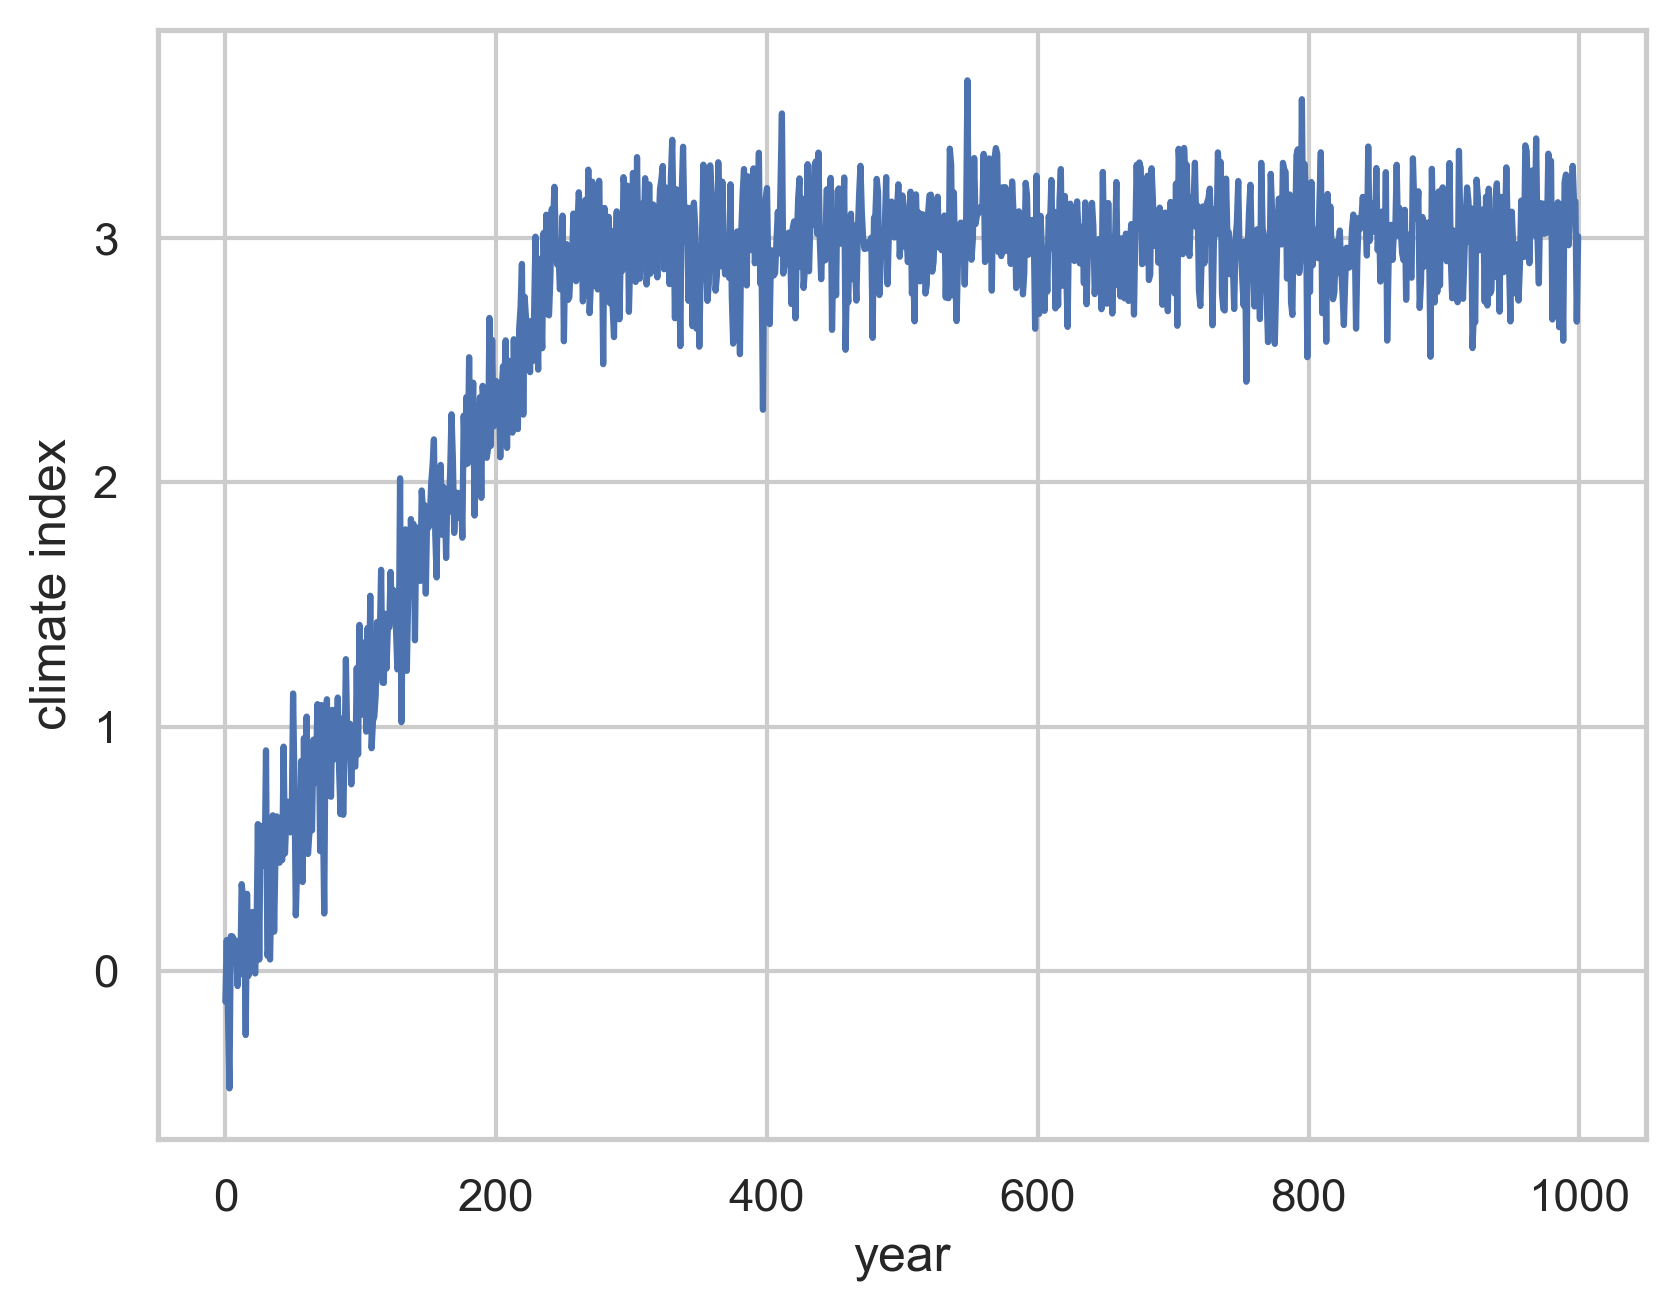
\includegraphics[width=0.6\textwidth]{../global-warming/figs/climate-index.png}
	\caption{The climate index spans \SI{1000}{\year}, and is provided as part of the glaciology course.}
	\label{fig:climate-index}
\end{figure}

\subsection{Idealized\_*}\label{app:forcing-idealized}

The idealized\_+12 forcing scenario is derived from an analysis of the climate index and the magnitude of the climate anomaly in 2100 CE, which is scaled by the climate index. Since the index peaks at \(\approx\num{3}\) and the temperature anomaly is \(\Delta T\approx\SI{4}{\celsius}\) (compare \cref{fig:era5,,fig:21c-warming}), increasing the temperature field by \(\Delta\mean{T}=\SI{12}{\celsius}\) yields a similar climate forcing as the NorESM case. Furthermore, \Textcite{greve2022} simulate the GrIS under a sustained late-21\textsuperscript{st}-century climate, hence, the temperature increase in the idealized\_+4 forcing is equal to the temperature anomaly in 2100 CE. This choice is within the projected window of global temperature rise in the RCP8.5, one of the pathways used by \textcite{greve2022}.

In both scenarios, changes in precipitation are neglected (\(\Delta P < \SI{0.2}{\mm\per\day}\)) and therefore computing of precipitation fields is unaltered.

\begin{figure}
	\centering
	\begin{subfigure}{0.46\textwidth}
		\centering
		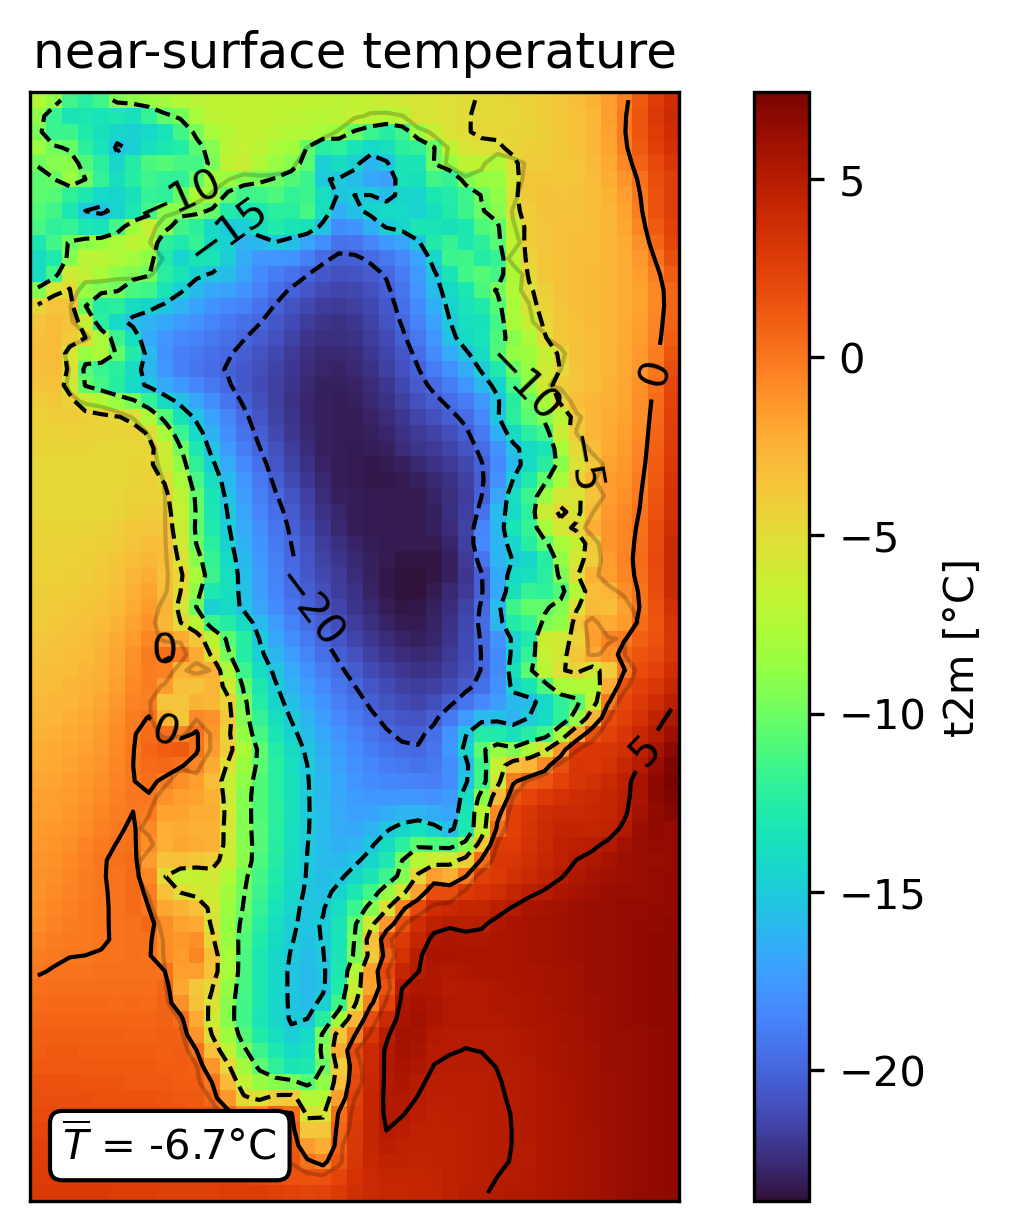
\includegraphics[width=\textwidth]{../global-warming/figs/21c-t2m-mean.png}
	\end{subfigure}
	\begin{subfigure}{0.44\textwidth}
		\centering
		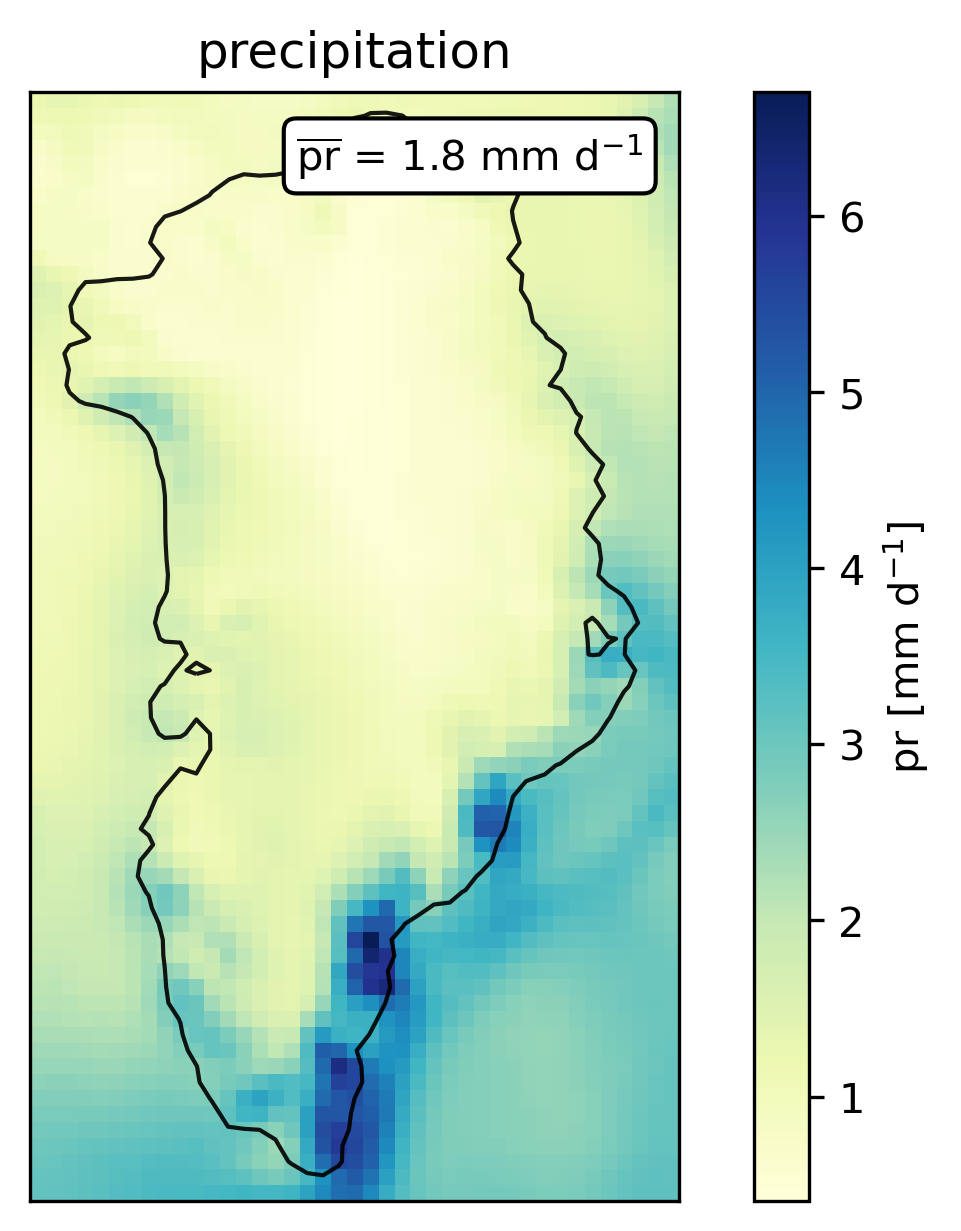
\includegraphics[width=\textwidth]{../global-warming/figs/21c-pr-mean.png}
	\end{subfigure}
	\caption{Annual mean near-surface temperature and precipitation for 2100 CE based on sum of projected anomalies by NorESM and present-day climatology}
	\label{fig:21c-warming}
\end{figure}
